\section{Comunicação}
Conforme explicado anteriormente, neste projeto utilizamos tanto protocolos de comunicação próprios quanto os elaborados comercialmente. A arquitetura desenvolvida aqui busca viabilizar a robustez do sistema, trabalhando em um nível local e outro nível remoto, onde o usuário terá o controle de sua casa por meio do \textit{smartphone} ou computador pessoal.

Nosso serviço em nuvem recebe as requisições do usuário por meio de um cliente web ou nativo. Esse servidor processa as requisições, aplicando os filtros de segurança necessários, de modo a consultar a autenticidade do pedido e verificar se aquele usuário possui as permissões necessárias para o serviço que deseja operar. Os serviços da nuvem se comunicam com o servidor local da casa requisitada, o qual também aplica os filtros de segurança necessários, e realiza a comunicação com os módulos.

A infraestrutura de comunicação entre a nuvem e o servidor local, e o servidor local e os sensores e atuadores utiliza o protocolo de aplicação \wmqtt{}, referência em aplicações IoT no mundo. O protocolo \wmqtt{} é estabelecido em cima dos protocolos TCP/IP (nas camadas inferiores) e é orientado à sessão, diferentemente do protocolo HTTP, de mesma camada.

O protocolo \wmqtt{} é do tipo Pub/Sub (de \textit{publisher/subscriber}) e é estritamente orientado à tópicos. Assim, um \textit{subscriber} se inscreve a um tópico de seu interesse, e recebe todas as publicações que um \textit{publisher} realizar. Os tópicos são organizados com estrutura semelhante a de um sistema de arquivos Unix, com níveis hierárquicos separados por barras, de modo que o subscriber pode se inscrever para tópicos utilizando \textit{wildcards} (* e +, os quais são válidos para mais de um nível e um único nível, respectivamente).

Para interconectar os tópicos, com \textit{publishers} e \textit{subscribers}, é necessário um agente que realiza a transmissão das mensagens, e que garante a segurança e confiabilidade. Esse agente é conhecido como Broker (em versões anteriores) ou Server (na versão atual, V3.1.1). O \textit{broker} irá permitir ou negar a subscrição ou a publicação a determinado tópico.

A segurança da troca de mensagens é realizada por meio do protocolo TLS (\textit{Transport Layer Security}) que encripta os segmentos na camada de transporte. Toda a parte de segurança e criptografia será detalhada no momento oportuno, bem como a organização dos tópicos implementados. % TODO era bom falar em qual seção está isso

Além disso, o protocolo \wmqtt{} oferece três tipos de QoS (\textit{Quality of Service}), possibilitando: diminuir o overhead ao máximo, enviando a mensagem uma única vez, na configuração mais simples; garantir que a mensagem seja entregue no mínimo uma vez, na configuração de segundo nível; garantir que a mensagem seja entregue exatamente uma vez, no terceiro nível, o que aumenta o overhead, consequentemente.

As mensagens são transmitidas em texto puro, e é necessário estabelecer um protocolo para a sua utilização. Utilizaremos aqui o protocolo que define a configurações das mensagens, desenvolvido no projeto HomeSky.

O \textit{broker} Mosquitto\footnote{https://mosquitto.org/} será utilizado, e foi escolhido por ser amplamente adotado em projetos de IoT, além de ser open source e com licença abrangente (MIT). Entretanto, há diversas possibilidades, como o HiveMQ, adotado no projeto HomeSky, e com grande uso em aplicações enterprise.

A arquitetura de comunicação é representada pelo diagrama abaixo, com um alto nível de abstração, cujos detalhes serão vistos no momento oportuno, com granularidade menor.

\begin{figure}[H]
	\centering
	\caption{Visão alto nível da comunicação no Hedwig}
  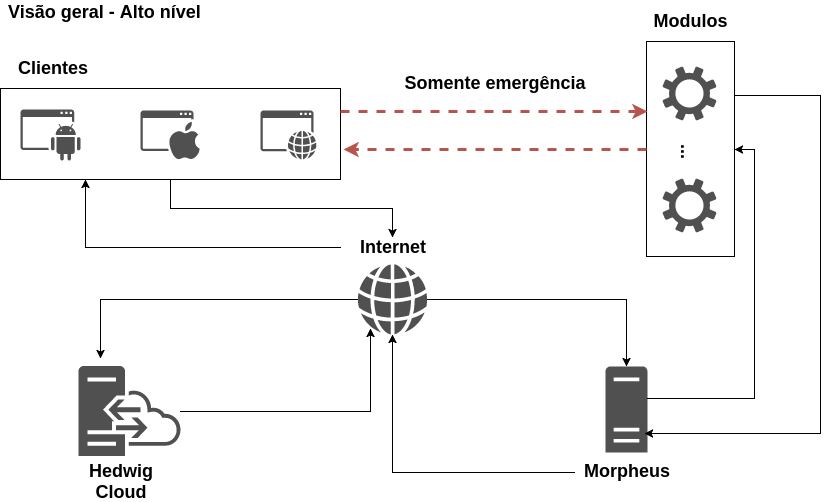
\includegraphics[width=0.8\textwidth]{arquiteturaHedwig}
\label{fig:diagramaComunicacao}
\end{figure}

\subsection{Entre módulos e controlador local}
\subsection{Entre controlador local e nuvem}
\subsection{Entre cliente web e nuvem}
\subsection{Entre app backup e módulos}
